\section{スズ-ゲルマニウム試料の作成と評価}
この章では電流パルス印加実験に用いた試料の作成法と、試料の評価結果を説明する。表\ref{tab:sample_results}にその内容をまとめた。

\subsection{合金(βスズ)試料の作成}
試料14は市販のスズショット(\textcolor{red}{東大??})を購入時のまま熱処理せず用いた。

そのほか合金試料の作成は理化学研究所吉川氏の指導のもと、理化学研究所の設備を用いて行った。まず、高純度の粒状のスズ(フルウチ化学SNM-67027A 純度99.999\%)と粒状のGe(フルウチ化学 GEM-33001A 純度99.999\%)をエタノールで超音波洗浄にかけた。そのあと洗浄したすり鉢でGeをすりつぶし粉状にした。それらの粒状スズとGeを以下に記述するように混合したあと、電気炉(\textcolor{red}{??})やアーク炉(\textcolor{red}{??})またはヒートガンを用いた三種類の手法で加熱し、常温まで冷却した。表\ref{tab:sample_results}の列[ 試料作成の条件 ]に作成条件を示す。

\subsubsection{封管試料の電気炉での加熱}
電気炉を用いた溶融法は温度履歴を管理できる点に強みがある。本実験ではGe濃度0.1 wt. \%(質量\%)、0.5 wt. \%、1 wt. \%の三通りについて、冷却速度をコントロールした試料を作成した。

試料1、2、3はそれぞれ、スズとGeがお互いに溶けあい均一な液相となったあと急冷した試料である。まず洗浄した粒状のスズ2gを電子天秤を用いて計量し石英管に入れたあと、Geが1 wt. \%(試料1)または0.5 wt. \%(試料2)または0.1 wt. \%(試料3)となるよう石英管に加えた。Ge粉末を石英管に入れる際は、静電気で石英管内面にくっつかないようにアルミ箔を細長く切って折りガイドにした。その後、石英管を真空ポンプで減圧し、石英管の中ほどを水素バーナーで加熱し封管した。図\ref{fig:GeSn_phase}のSn-Ge合金試料の相図によると、Sn-Ge合金試料はその組成によらず1000℃を越えると完全に溶解する。電気炉で封管された石英管ごと試料1、2、3を加熱し、1050℃に達したあとよくふって混合して、石英管のまま水の中に浸して急冷した(水クエンチ)。この際、冷却し固化するのにかかる時間スケールは10秒程度であった。

試料6はスズとGeがお互いに溶けあい均一な液相となったあと徐冷した試料である。試料1、2、3と同様に試料6もGeが1wt.\%濃度となるよう混合し、電気炉を用いて1050℃まで加熱したあと、48時間かけて室温まで徐冷した。

試料4は、スズとGeがお互いに溶けあわない不均一な状態で急冷した試料である。試料1,2,3,6と同様に混合したあと、スズ単体の融点とGe単体の融点の間の400℃まで加熱し、石英管を水の中に浸し急冷した。スズとGeは室温で分離しているため、スズ液相中にGeが溶け込むには時間がかかる。それをあえて待たずに水クエンチした。

試料5ではスズとGeの界面の状態を観察するために、粒状スズと粉末Geを質量比1:1で1gずつ混合した。それらをスズ単体の融点とGe単体の融点の間の400℃まで加熱したあと、急冷した試料である。こちらも試料4と同様に、不均一な状態で水クエンチした。

\subsubsection{アーク炉での加熱}
アーク炉の内は温度分布が一様でなく温度履歴を管理できないが、アーク炉を用いた溶融は簡便である。本実験ではGe濃度0.1 wt. \%、1 wt. \%の二通りについて、アーク炉の出力を変化させた。

試料7、8は、試料1、2、3と同様にスズとGeがお互いに溶けあったあと急冷することを目指した試料である。一方、アーク炉のサンプルステージは熱伝導のよい銅でできており絶えず水で冷却しているので、速い冷却速度が期待できる。Ge濃度が1 wt. \%(試料7)と0.1 wt. \%(試料8)となるように粒状スズと粉末Geを混合したあと、サンプルステージに置き、電極を近づけアーク電流を最大出力で流したあと、電流を切った。

試料9、10はアーク炉の出力を半分以下とした点以外、試料7、8と同様である。Ge濃度が1 wt. \%(試料10)と0.1 wt. \%(試料8)となるよう同様に混合したあとサンプルステージに置き、電流を最大出力の半分以下で流したあと、電流を切った。試料4と同様に、スズとGeがお互いに溶けあわない不均一な状態で急冷された。

\subsubsection{ヒートガンでの加熱}
ヒートガンは小型の簡単な熱源であるため400℃以上の高温には到達できないが、アーク炉に比べてさらに簡便である。ヒートガンを用いた簡便な試料作成法が確立できれば、気軽に様々な場所で試料作成できて作成条件の最適化に向いている。本実験ではGe濃度0.1 wt. \%(質量\%)、0.1 wt. \%、0 wt. \%の三通りについて、試料を作成した。

試料11、12、13を作成する際は、試料1、2、3、6と同様に粒状スズと粉末Geを石英管に入れた。その石英管を真空ポンプで減圧した状態でヒートガンを押し当てて加熱し、スズが液体となったら加熱をやめ空気中で放冷した。

\subsection{合金(βスズ)試料の観察・評価}
溶融・冷却後、前節に記述した11通りのAs grown試料を外見から観察した。さらにそれぞれダイアモンドカッターで切断して、内部も観察した。表\ref{tab:sample_results}の列[ As grown試料の見た目 ]に観察結果を示す。さらに試料1、2、3、6に関してはX線回折測定から構造を確かめた。

\subsubsection{As grown試料の観察結果}
試料1、2、3、6、7、8、\textcolor{red}{9、10、11、12}を観察したところ表面は滑らかであり、銀色の光沢があった。また切断面から内部を見ても均一だった。

試料4はGeとスズを質量比1:1で混合し電気炉で400℃まで加熱したあと急冷した試料であるが、Ge粒の隙間を埋めるようにスズが溶け込んでいた。

試料5はGeが表面に塊のまま分布しており、空間的にGe濃度が不均一だった。しかしGe粉末がついた層から離れた内部は均一だった。

試料6の表面は大きくへこんでいた。図\ref{fig:sample6_asgrown}に試料6の外見を示す。このようなくぼみは他の試料には見られなかった。しかし切断し内部を観察すると、一様な見た目をしていた。
\begin{figure}[!h]
    \begin{center}
   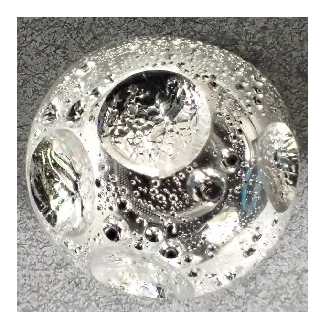
\includegraphics[width=0.4\hsize]{samples/sample6_asgrown.eps}
  \end{center}
  \caption{徐冷中に表面が大きくへこんだ試料6(Ge1wt.\%)}
  \label{fig:sample6_asgrown}
\end{figure}

試料13は表面が滑らかで光沢があるが、黄色い層が表面にあった。

試料14の表面には傷があるが、光沢があった。

\textcolor{red}{外見と内部に関しては実際の試料を確認する。細かく観察する。}

\subsubsection{合金(βスズ)試料のX線回折測定}
As grownのβスズ試料についてX線回折測定を行い、結晶構造を解析した。測定には理化学研究所のX線回折装置(Rigaku\textcolor{red}{??})を用いた。

X線源には熱電子が銅ターゲットで制動放射される際に出る$\rm CuK\alpha$線(特性X線)を用い、基板には多結晶のガラスを用いた。測定は$\rm 2\theta/\theta$配置で行った。図に$\rm 2\theta/\theta$配置の入射光と試料と回折光の位置関係の模式図を示す。X線は試料に入射角$\rm \theta$で入射し、Braggの回折条件$2d\:sin\theta=\lambda$を満たすとき、出射角$\rm \theta$で回折する。ただし$d$は基板に平行な格子面間隔であり、$\lambda$は特性X線の波長である。したがって角$2\theta$は回折角度に対応する。$\rm 2\theta/\theta$配置ではX線検出感度を高くできる。
\begin{figure}[!h]
    \begin{center}
   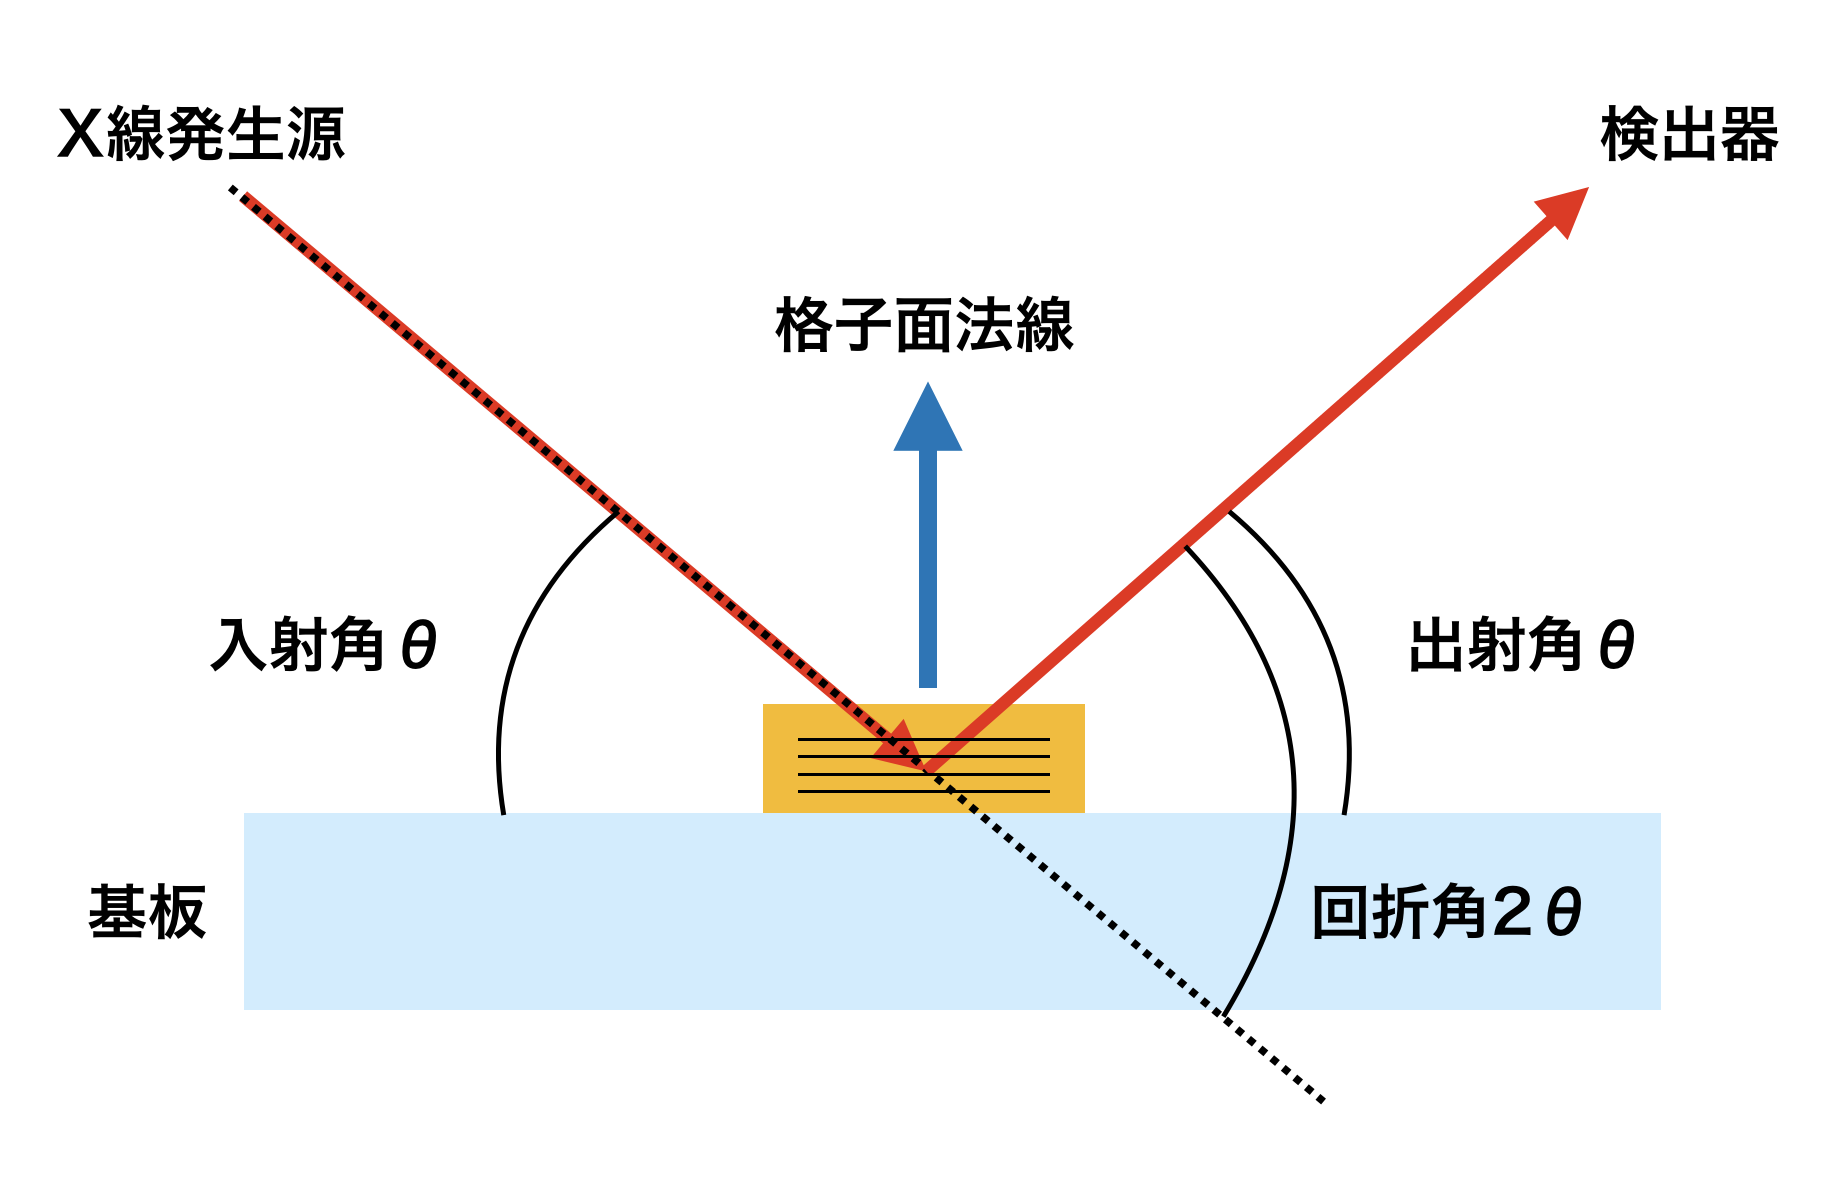
\includegraphics[width=0.6\hsize]{experiment/schematics_Xray.eps}
  \end{center}
  \caption{X線回折測定($\rm 2\theta/\theta$配置)の模式図}
  \label{fig:schematics_Xray}
\end{figure}

試料の結晶構造を精度よく同定するためには、試料がX線源と検出器の光軸が交わる領域に存在し、高さ方向に基板から出っ張っりすぎていない必要がある。

図\ref{fig:intensity_asgrown_samples}に、試料1、2、3、6の回折強度を$2\theta$に対してプロットしたものを示す。また空間群の対称性をもつβスズの室温での(293K)での格子定数a=b=5.8303 Aとc=3.1810A \cite{Wolcyrz}から、粉末X線回折スペクトルを再現した図も併せて示す(beta-Sn)。
\begin{figure}[!h]
    \begin{center}
   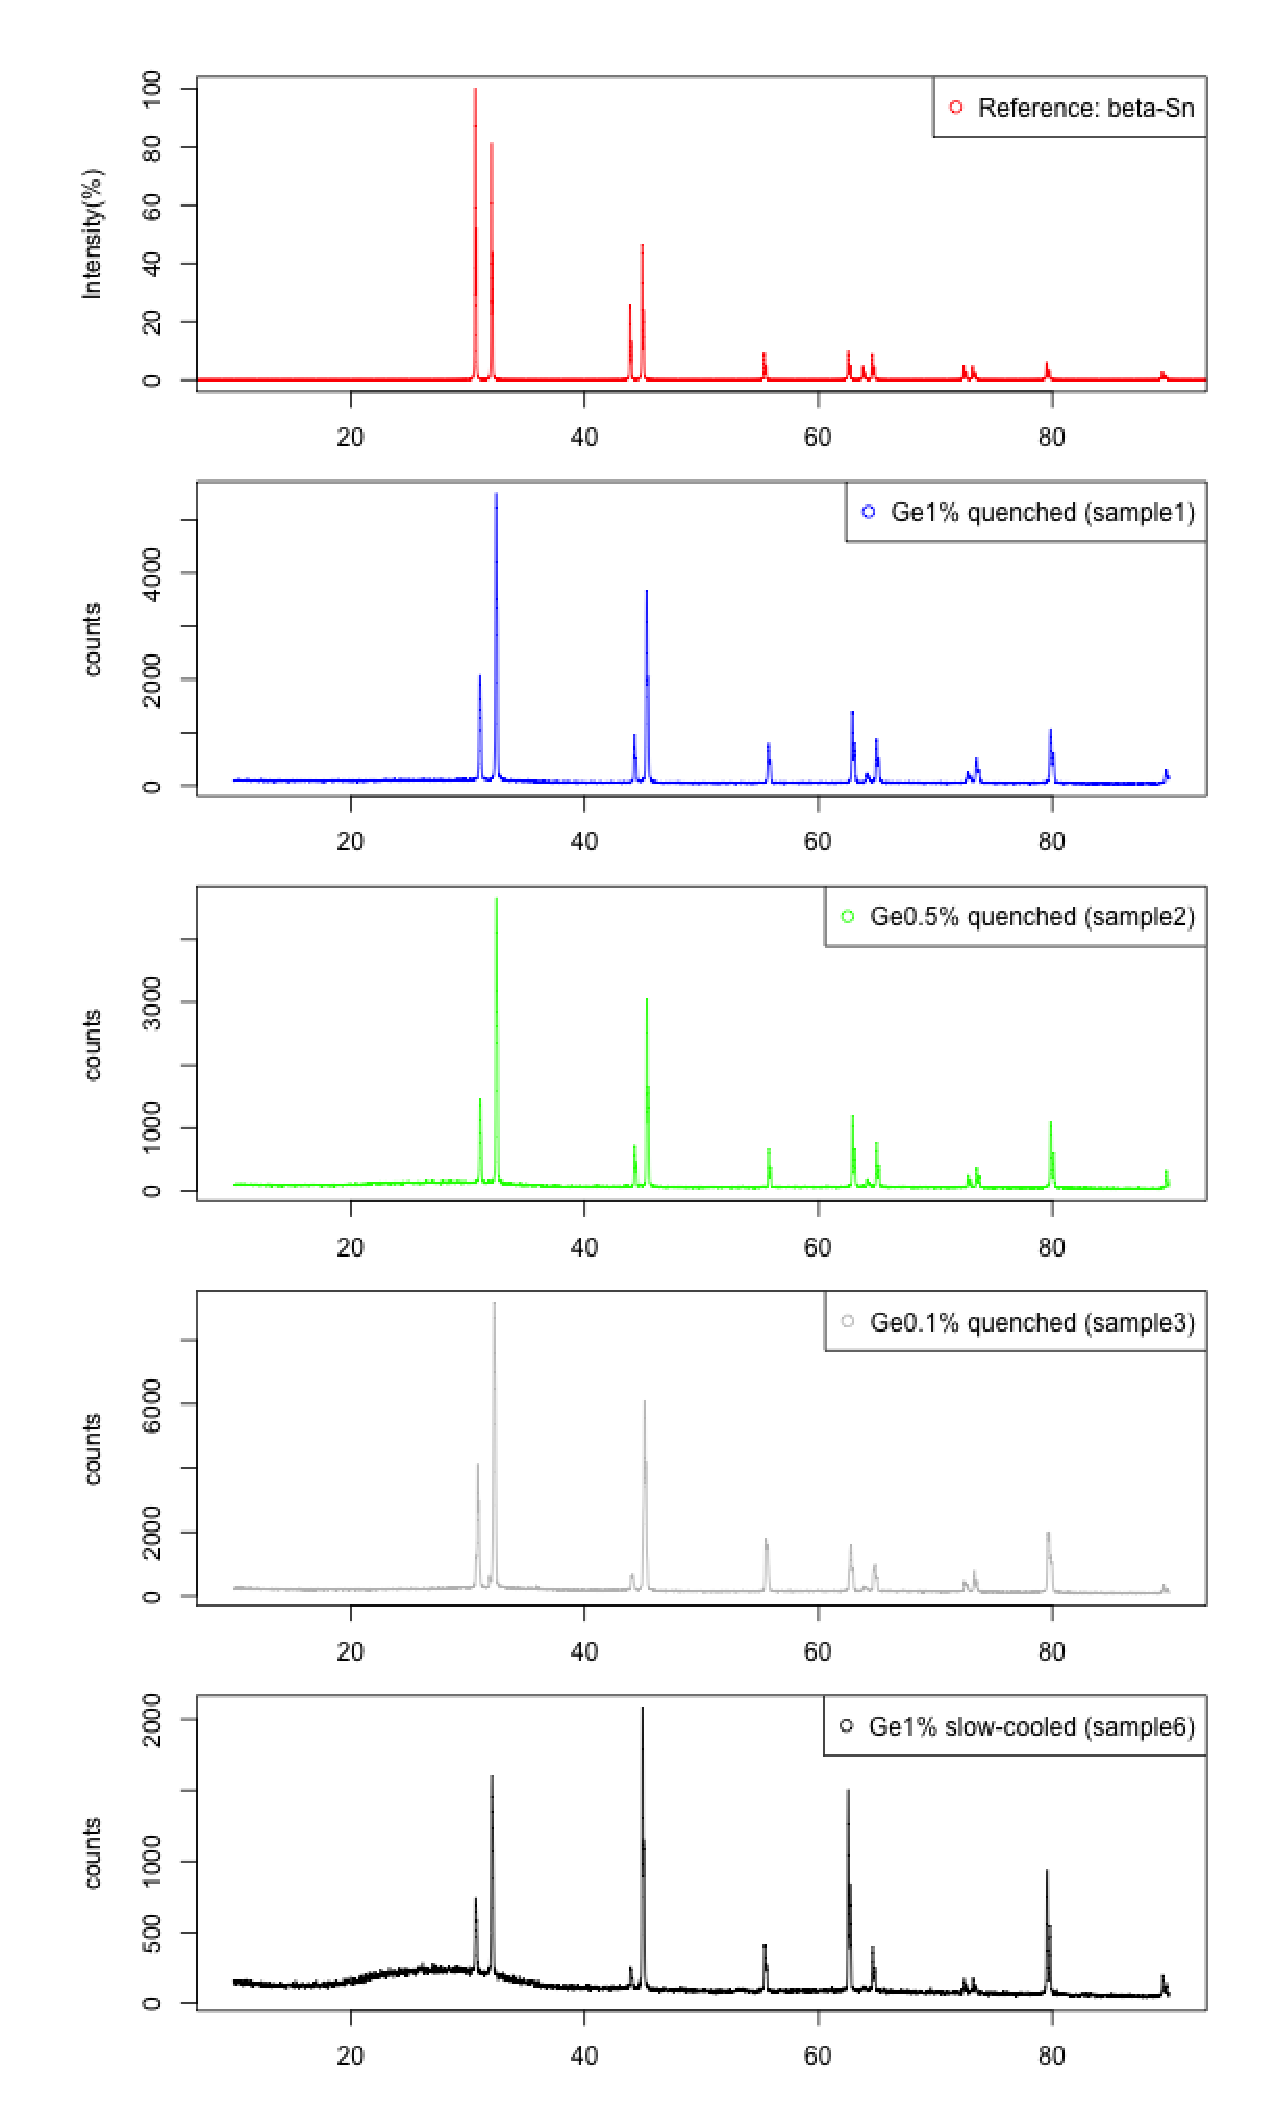
\includegraphics[width=\hsize]{samples/intensity_asgrown_samples.eps}
  \end{center}
  \caption{As grown(β相)試料}
  \label{fig:intensity_asgrown_samples}
\end{figure}

それぞれの試料に対して、βスズの粉末X線回折で現れる全てのピークが見えている。すなわち、試料はそれぞれβスズと同一の構造を持った多結晶を含むことが分かる。またGeやαスズに由来する回折のピークは見られず、大部分がβスズであることを確かめた。なお試料6において、$2\theta=20^\circ$から$2\theta=40^\circ$にかけて、ブロードな回折が見られる。測定した試料6は小さかったため、アモルファス構造を持つ基板の石英ガラスのハロー回折\cite{Speakman}が見えている。しかしこのブロードなスペクトルの影響は小さいため無視できる。

\subsection{半導体(αスズ)試料への変換}
本研究の目的である半導体スズと超伝導体スズとの変換を達成するためにはパルスを用いてβスズをαスズに変換するだけではなく、αスズをβスズに変換しなければならない。また序論で述べたようにαスズをβスズに変換する方が逆の過程に比べ、かかる時間が短く簡便である。したがって筆者はいずれβスズに再度変換することを目的として、一部のAs grownのβスズ試料を(パルスを用いない準静的な過程により)αスズに相転移させた。

βスズからαスズへの相転移は230Kから260Kでおきる\cite{Matvienko,Ogino,Cornelius}ため、家庭用冷蔵庫の冷凍室($\rm<$255K)をその際の保管庫として利用できる。筆者はβスズ試料をダイアモンドカッターを用いてスライスして測定に適した形状に加工したのち、冷凍庫に保持しβスズからαスズへの相転移を観察した。またその際の相転移にかかった時間をおおまかに記録した。表\ref{tab:sample_results}の列[ β$\to$α転移にかかる時間] にβスズからαスズへの転移にかかった時間をまとめる。

\subsubsection{試料6}
試料6はカットしたAs grown試料を2つ用意し冷凍庫の中に保持した。1つはカットした際のバリから核生成して3日以内に相転移が完了し、バリのないもう1つは3日以内に核生成しなかった。

この違いはバリから核生成が始まった事実から説明できる。試料はα-β相転移する際に27\%程度の体積変化を伴うため、試料の核生成は試料の内部より表面から始まりやすく、また表面よりもエッジから始まりやすい\cite{Cornelius}。したがって、尖ったエッジやバリ、傷のある試料はそうでないものに比べ核生成しやすい。

\subsubsection{試料1}
試料1のAs grownでは3週間($\sim$500h)経っても転移しなかった。

そこで、まず筆者は試料1では何らかの理由でαスズの核が生成されていないのではないかと仮説を立てた。核生成は試料の内部より表面やエッジから始まりやすい\cite{Cornelius}ため、試料6で確認したように、傷をつけた試料の方がAs grown試料より核生成しやすい。筆者は試料1の表面にカッターナイフで傷を入れたり、ニッパーで切り込みを入れることで核生成を促進しようとした。またαスズに変換するためにαスズそのものや、GeやSiのようなαスズと同じダイアモンド構造などをβスズに押し付けると、その部分から相転移が始まりやすいことが知られている\cite{Cornelius}。さらに筆者はすでに転移していた試料2のα相を試料1に押し付けて、核生成を促進しようとした。

しかしそれらの工夫をしても数週間程度で相転移の進行は確認できず、3ヶ月間放置することで相転移が完了していることを確認した。

核生成しても相転移に数週間程度以上の時間がかかるこの結果は、核生成以外の要因により相転移が阻害されている可能性を示唆する。
Matvienkoら\cite{Matvienko}によるとβ$\to$α転移はβスズの塑性変形が重要な役割を果たすが、その塑性変形に伴う欠陥の拡散を分散したGeが阻害するため、Geの添加はαスズへの転移速度を遅くする(図\ref{fig:Ge_content})。この結果によって、Geを1 wt. \%添加し急冷した試料1の相転移が非常に遅く相転移を数週間程度で観察できなかった理由が説明できる。
\textcolor{red}{詳しく書けるように勉強する}

\subsubsection{試料6と試料1の比較}
試料6は3日程度で相転移したのに対し、試料1は短くとも数週間程度以上が相転移にかかった。これら2つの試料はともにGeを1 wt. \%添加し、電気炉を用いて1050℃まで加熱した。作成条件の差は試料作成時の冷却速度のみである。

筆者は冷却速度の違いにより、Geの相分離の程度または空間分布が異なるのではないかと仮説を立てた。

スズ 99 wt. \%-Ge 1 wt. \%合金は平衡状態にあるとき相分離する。
Ge-スズ合金の平衡相図を表した図\ref{fig:GeSn_phase}とそのGeリッチ領域を拡大した図\ref{fig:GeSn_phase2}によると、スズ 99 wt. \%-Ge 1 wt. \%(スズ 98.4 at. \%-Ge 1.6 at. \%)合金が室温で平衡状態にあるとき、スズ 98.4 at. \%のスズと1.6 at. \%のGe(0.5 at. \%のスズを固溶)は分離して存在する。量比の計算にはてこの原理を用いた。試料6が平衡状態にあると仮定すると、スズリッチな領域はほとんどGeを固溶していない(0.3\%以下\cite{Thurmond1960})。

試料6が平衡状態になく偏析しているとしても、Ge濃度が空間分布しているという議論は変わらない。図\ref{fig:GeSn_phase}、\ref{fig:GeSn_phase2}によると、冷却中の330℃程度で、融液はスズを1.1at.\%程度固溶したGeを初晶として晶出し始め、融液のGe濃度は減少してゆく。共晶温度231.1℃まで融液を冷やしたとき、融液のGe濃度は共晶組成のGe濃度0.26 at. \%程度\cite{Thurmond1960}まで落ち込む。その濃度でさらに共晶反応が起こり、融液がSnリッチな領域とGeリッチな領域に分離して固化する。したがって平衡状態になく偏析していたとしても、試料6の相分離したSnリッチ領域はGeを0.26 at. \%以下しか含まない。
%Ge:Snを原子数比でx:(1-x)、質量比でX:(1-X)とすると、ゲルマニウムの原子番号32とスズの原子番号50から
%X=32x/[50(1-x)+32x]; x=50X/[50X+32(1-X)]

一方、10秒程度の時間スケールで急冷した試料1に関しては相分離は起こらない(\textcolor{red}{要出典/EdX})。したがって試料1においてGe濃度は空間的に一様である。
\textcolor{red}{根拠を明確にする必要がある}

\subsubsection{試料2、3、11、12}
試料2、3、11、12はいずれも1週間($\sim$170h)または2週間($\sim$340h)以内でαスズへの転移が終了した。ただしこれは筆者が冷凍庫に試料を入れて1週間後または2週間あとに再び開けたときに転移していたという意味であり、実際は数時間程度で転移が完了していた可能性もあることに注意する。

転移した後の試料の見た目(割れ方)は異なる。図\ref{fig:diff}に試料2、3、11、12のβ$\to$α相転移前後の外観の変化を示す。転移後の試料2、3は数カ所程度の亀裂しか入っていないのに対し、試料11、12は粉々に砕けている。
\begin{figure}[!h]
    \begin{center}
   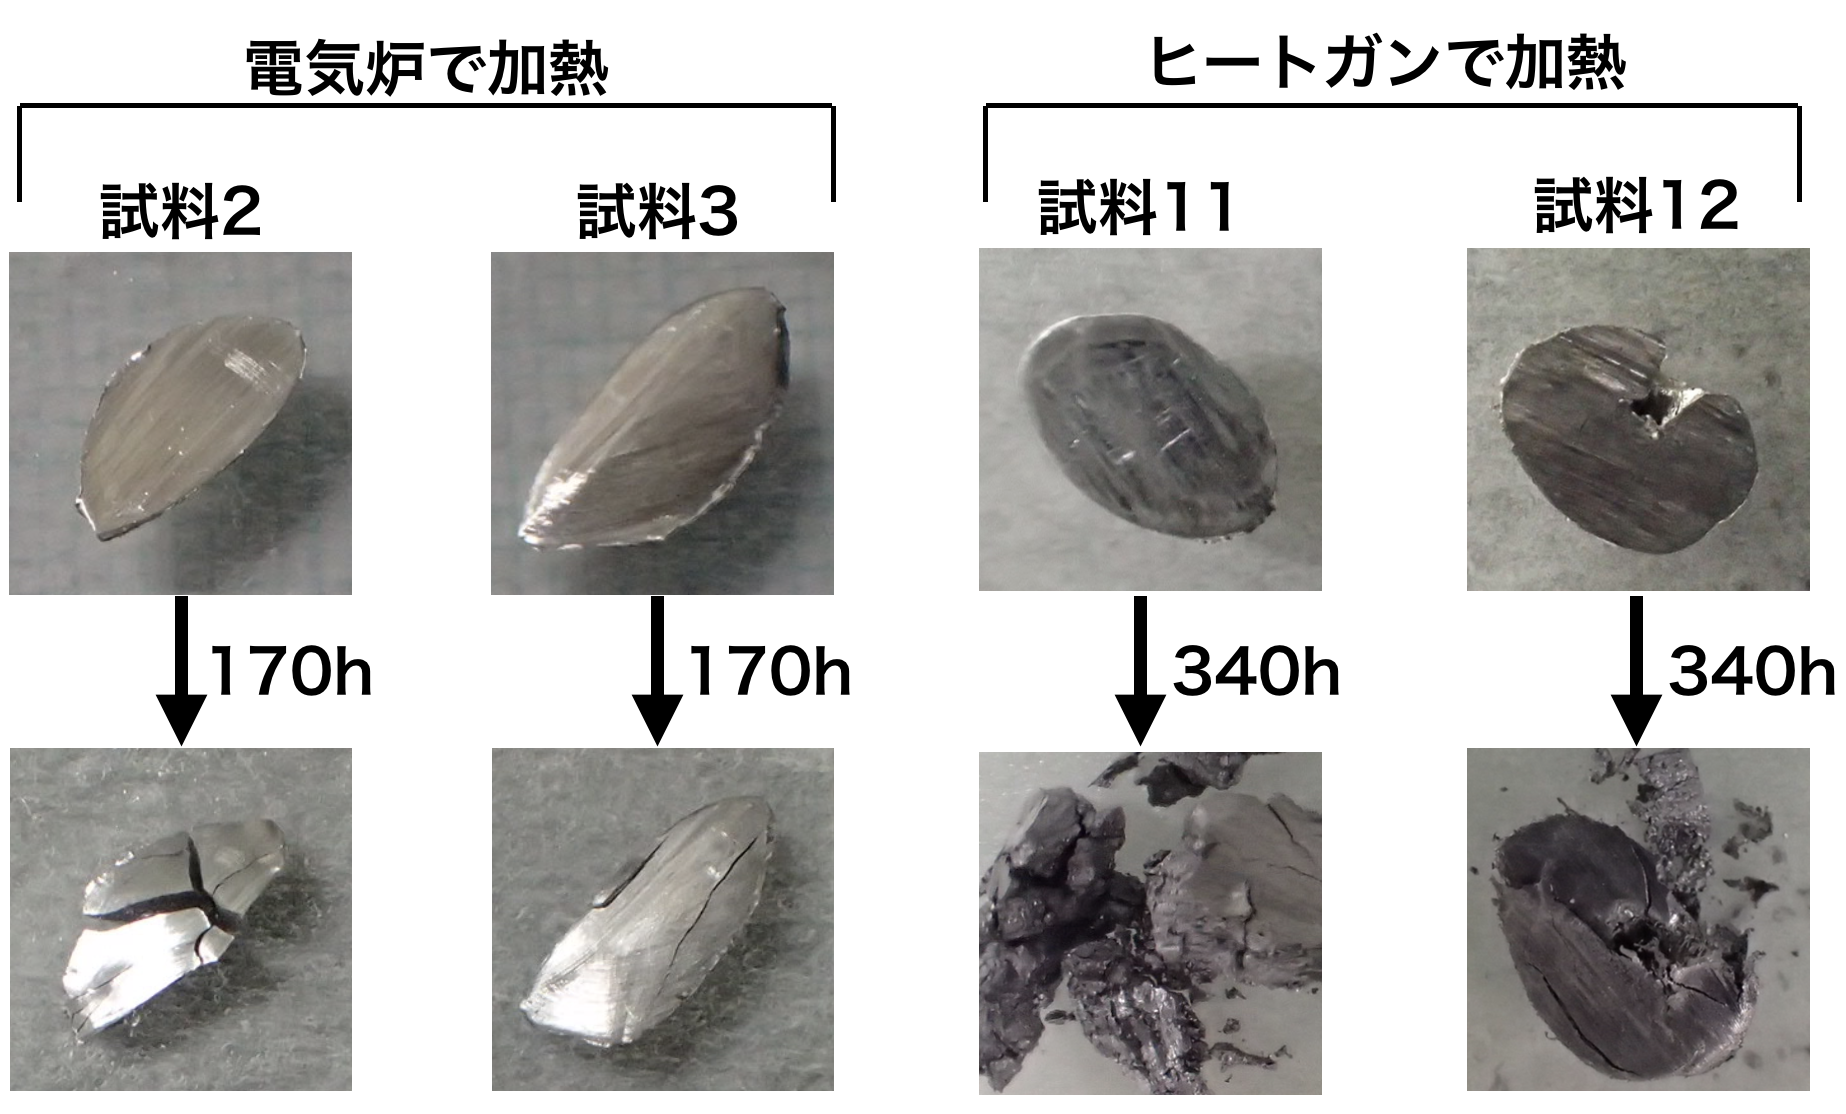
\includegraphics[width=0.6\hsize]{samples/diff.eps}
  \end{center}
  \caption{β$\to$α相転移前後の外観の変化}
  \label{fig:diff}
\end{figure}

筆者は転移の際の割れ方の違いがGe分布の違いによるものであると考える。電気炉で1050℃まで加熱したあと急冷した試料2と3はGe濃度が空間的に一様であるため局所的な強い内部応力は起こりにくい。一方ヒートガンで加熱した後放冷した試料11と12はGe溶けきっておらずが内部に侵入しているので、そこを核としてβ$\to$α相転移し膨張する。結果として内部から強い応力がかかった状態で転移するので粉々になるのではないだろうか。

%\subsubsection{試料4、5、7、8、13、14}
\subsubsection{試料13、14}
Geを含まない試料13と試料14をAs grownの状態でそれぞれ2週間と半年間冷凍庫に保持したが、ともに相転移しなかった。Geを添加し転移した他の試料と比較すると、際立った特徴である。Geを添加することはβ$\to$α転移を促進するために有益であることを確かめた。

\subsection{試料7、8}
Geを1 wt.\%含む試料7は1週間で相転移したが、1 wt.\%の試料8は1週間で転移しなかった。
Ge量とβ$\to$α転移転移に関する評価は今後の課題である。

\subsection{試料5}
Geが不均一に分布した試料は相転移した。その相転移に関する評価は今後の課題である。

\subsection{半導体(αスズ)試料の観察・評価}

\textcolor{red}{試料6はゆがんだ層状の構造が見て取れて、薄い薄片状のサンプルが見つかった。(画像)}
\textcolor{red}{EdXが必要ならする}
%\subsubsection{半導体(αスズ)試料のEdX}

\subsubsection{半導体(αスズ)試料のX線回折測定}
$\rm 2\theta/\theta$配置において室温でαスズに変換された試料のX線回折強度を測定し、試料の構造解析を行った。αスズの試料は割れていて小さいので固定が難しく、基板の上に置くと出っ張ってしまう。そこで炭酸カルシウムを主成分とする粘土に埋め込み、平らな面を上にしてX線を入射した。

図\ref{fig:intensity_pested_samples}に、試料2、3の回折強度を$2\theta$に対してプロットしたものを示す。また空間群$aa$の対称性をもつαスズの室温での(293K)での格子定数a=b=c=6.4892\AA \cite{THEWLIS}から、粉末X線回折スペクトルを再現した図も併せて示す(alpha-Sn)。さらにリファレンスとして、測定した炭酸カルシウムの回折強度(CaCO3)を示す。
\begin{figure}[!h]
  \begin{center}
  \includegraphics[width=\hsize]{samples/intensity_pested_samples.eps}
  \end{center}
  \caption{α相に変換された試料}
  \label{fig:intensity_pested_samples}
\end{figure}

それぞれの試料の回折強度には、αスズまたは炭酸カルシウムに由来するピークが現れている。したがって冷凍庫に保持した後、as grown試料には見られなかったαスズが現れたことが分かる。またGeやβスズに由来する回折のピークは見られないため、大部分がαスズであることが言える。

回折強度がところどころが負になっている理由は、主に二つあると筆者は考える。一つ目はリファレンスの強度が適正な値より大きくなっていることである。試料を取り外し炭酸カルシウム粘土のレフェレンスを測定する際、試料が覆っていたところにもX線が入射する。したがって試料以外からの寄与は大きく見積もられる。二つ目は試料の高さがわずかに変化した影響である。この効果はリファレンスを引き算するとき、影響が大きい。
回折角$\rm 2\theta$しかしこれらの問題点は、冷凍庫で保持した後のスズのうちがαスズの構造が支配的であるとする筆者の結論に影響を与えない。
Oxford \textcolor{red}{文章は後回し/図も書いたほうがいい}


\subsection{α相からβ相への転移温度}
スズはα-β相転移の前後で抵抗が大きく変化する。試料2、3、6、7について加熱しながら抵抗測定を行い、抵抗変化から相転移温度を見積もった。抵抗測定は横磁場クライオスタット(Oxford \textcolor{red}{??})を用いて、通常の4端子法により行った。

試料2、3、6の抵抗の温度依存性を図\ref{fig:Trans}に、試料5、7の抵抗の温度依存性を図\ref{fig:Trans2}に示す。ただし抵抗は温度300Kの値で正規化した。

どの試料も温度を上げてゆくと緩やかに抵抗が現象してゆくが、ある温度領域から急激に抵抗値が小さくなる。これは半導体のαスズが金属のβスズに結果であると考えられる。どの試料も転移した後、温度が小さくなるにつれて温度に対し線形に抵抗が減少した。この抵抗の温度依存性は金属的である。

落ち込む前と落ち込んだ後の抵抗の間の抵抗値をとる温度を相転移温度$\rm T_c$と見積もって、図\ref{tab:sample_results}の列[ $\alpha\to\beta$転移温度 ]に示す。また相転移が始まった温度と終わった温度の差を抵抗変化から読み取って$\rm \Delta T_c$として、併せて示す。

試料1の転移オンdお
試料2はともにだった。

試料3はともに

試料7-1と7-2はともに。Geが空間的に不均一に入っていることがわかる。

\begin{figure}[!h]
 \begin{minipage}{\hsize}
    \begin{center}
   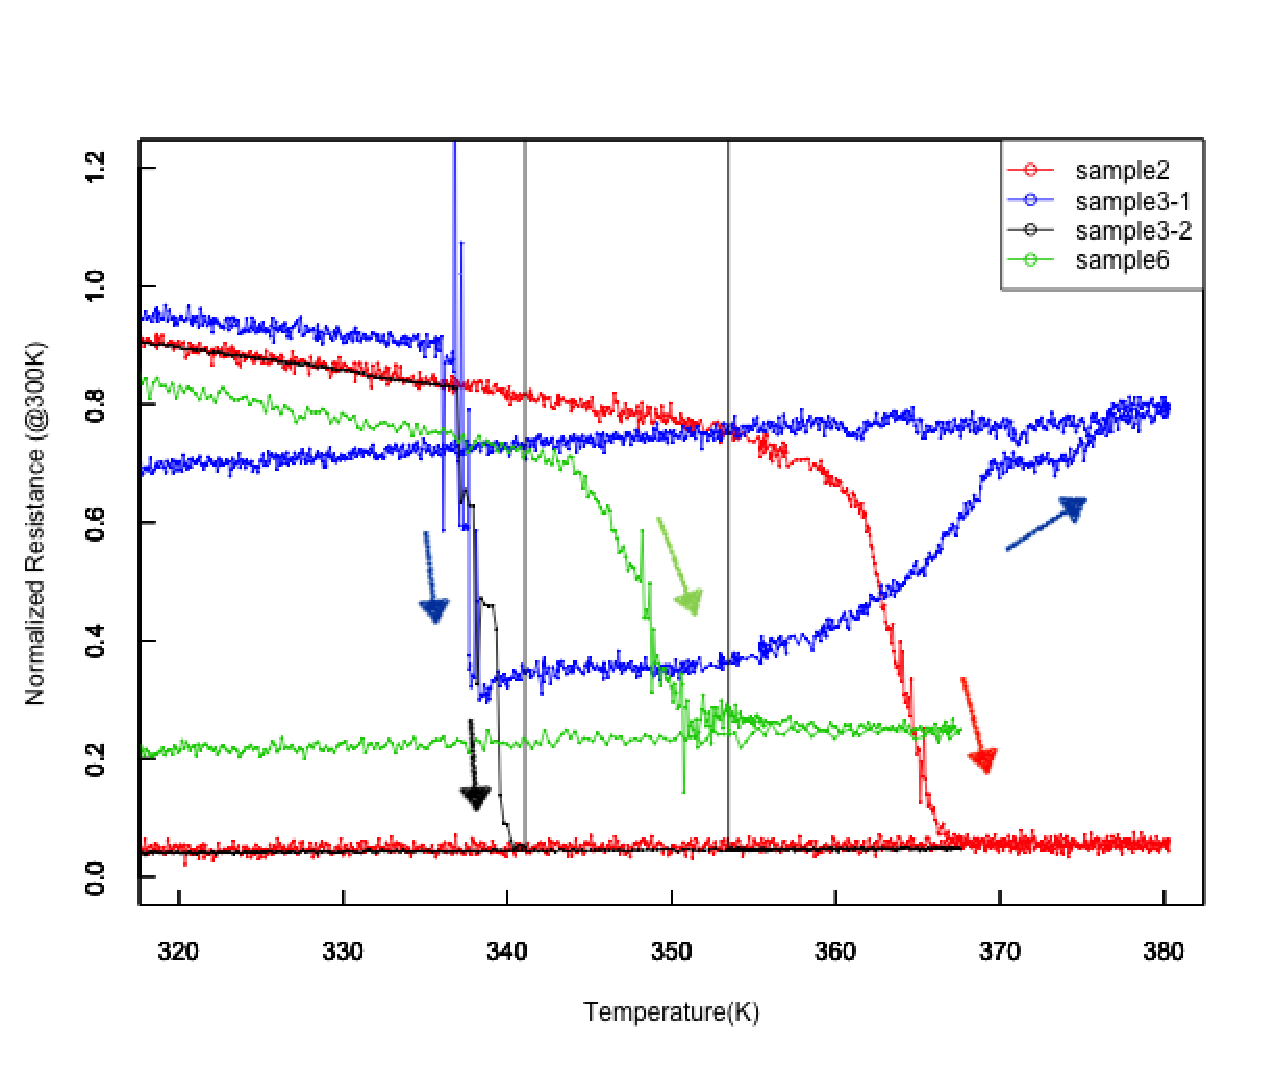
\includegraphics[width=0.9\hsize]{samples/Trans.eps}
  \end{center}
  \caption{}
  \label{fig:Trans}
 \end{minipage}
 \begin{minipage}{\hsize}
     \begin{center}
   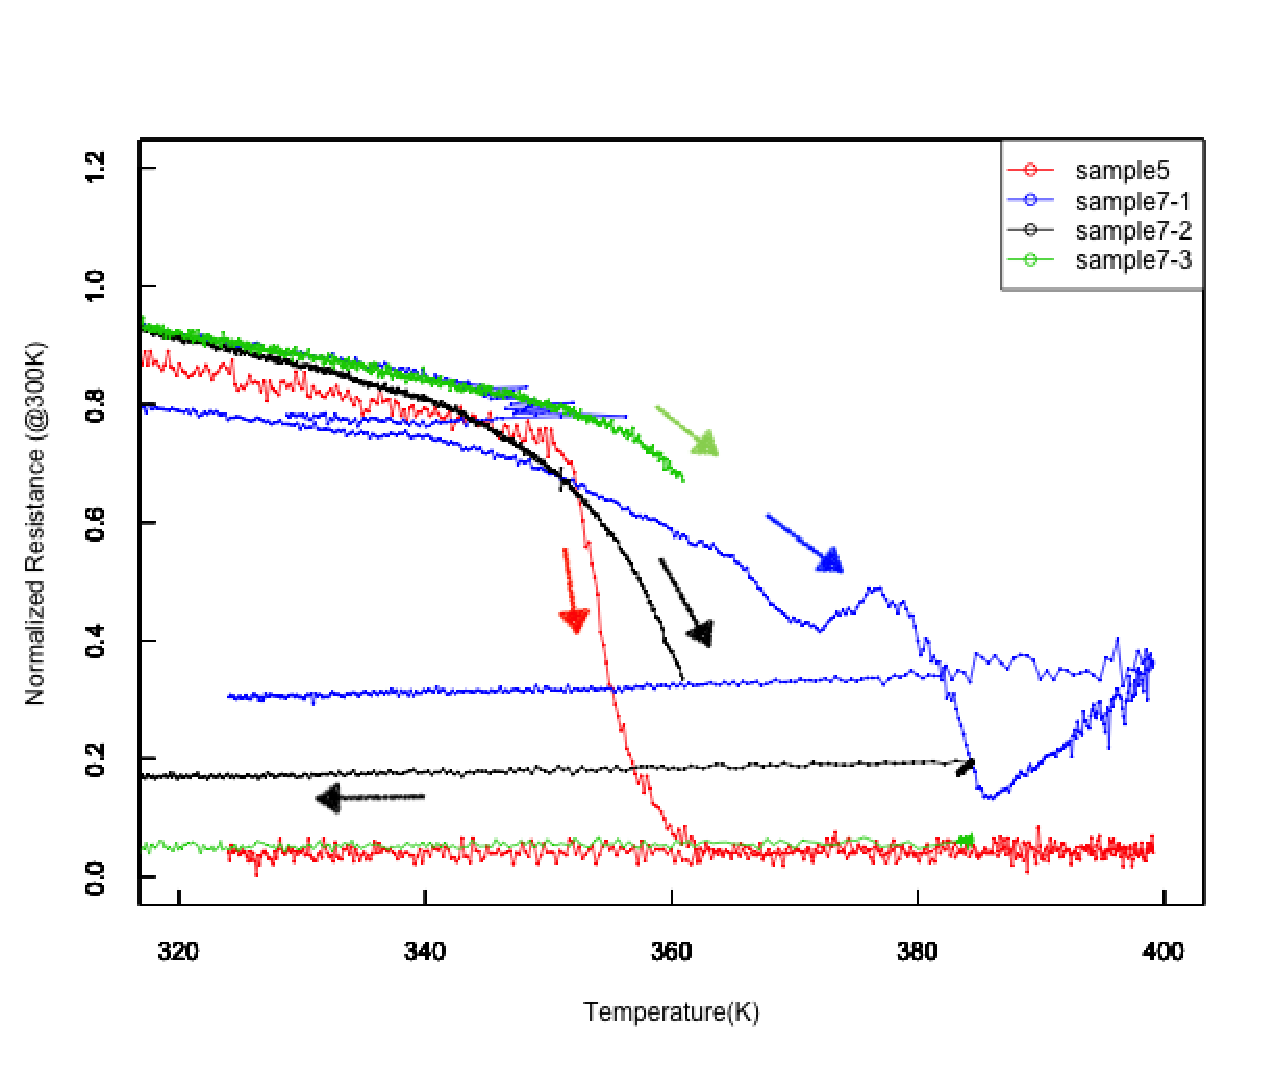
\includegraphics[width=0.9\hsize]{samples/Trans2.eps}
  \end{center}
  \caption{}
  \label{fig:Trans2}
   \end{minipage}
\end{figure}

Oxford \textcolor{red}{もう少し補足説明があったほうがいい}

\begin{landscape}
\begin{table}[!h]
    \begin{center}
  \begin{tabular}{c|cccc|cc|ccc|cc}
&  \multicolumn{4}{|c|}{試料作成の諸元}& \multicolumn{2}{|c|}{As grown試料の見た目}&\multicolumn{3}{|c|}{β$\to$α転移にかかる時間(h)}&\multicolumn{2}{|c}{$\alpha\to\beta$転移温度(K)}\\
No.&Ge-wt.\%&溶融法&到達温度/出力&冷却法&表面&内部&As grown&傷つけ&Ge押し付け&$\rm T_c$&$\rm \Delta T_c$\\ \hline
1&1.0&電気炉&1050℃&水クエンチ&滑らか&一様&$>$500*&170$\sim$2200&170$\sim$2200&&\\
2&0.5&電気炉&1050℃&水クエンチ&滑らか&一様&$<$170&&&364&5\\
3&0.1&電気炉&1050℃&水クエンチ&滑らか&一様&$<$170&&&338.5&4\\
4&50&電気炉&400℃&水クエンチ&\multicolumn{2}{|c|}{(図注に別記)}&&&&&\\
5&1.0&電気炉&400℃&水クエンチ&Ge粉末&不均一&$<$170&&&&\\
6&1.0&電気炉&1050℃&徐冷(48h)&くぼみがある&一様(層状?)&$<$72&&&347&6\\
&&&&&&&$>$72*&$<$48&&&\\
7&1.0&アーク炉&最大出力&急冷&&&$<$170&&&&\\
8&0.1&アーク炉&最大出力&急冷&&&$>$170*&&&&\\
9&1.0&アーク炉&半分以下&急冷&&&&&&&\\
10&0.1&アーク炉&半分以下&急冷&&&&&&&\\
11&1.0&ヒートガン&&放冷&&&$<$340&&&&\\
12&0.1&ヒートガン&&放冷&&&$<$340&&&&\\
13&0.0&ヒートガン&&放冷&滑らかな黄色&&$>$340*&&&&\\
14&0.0&(熱処理なし)&&&&&$>$4400*&&&&\\
  \end{tabular}
  \caption{実験結果の比較($\rm \Delta T_c=T_f-T_i$は抵抗測定で抵抗が落ち始めた温度$\rm T_i$と終わった温度$\rm T_f$の差。列 β$\to$α転移にかかる時間における記号*は相転移しなかったことを表す。)}
  \label{tab:sample_results}
    \end{center}
\end{table}
\end{landscape}
%2日=24*2h=48h/ 3日=24*3h=72h/ 1週間=24*7h=168h/ 2週間=24*14h=336h/ 3週間=24*21h=504h/ 1ヶ月=24*30h=720h/ 3ヶ月=24*91h=2184h/ 6ヶ月=24*365/2h=4380h

\clearpage


